\section{Bildschirm}
\begin{figure}[h]
    \centering
    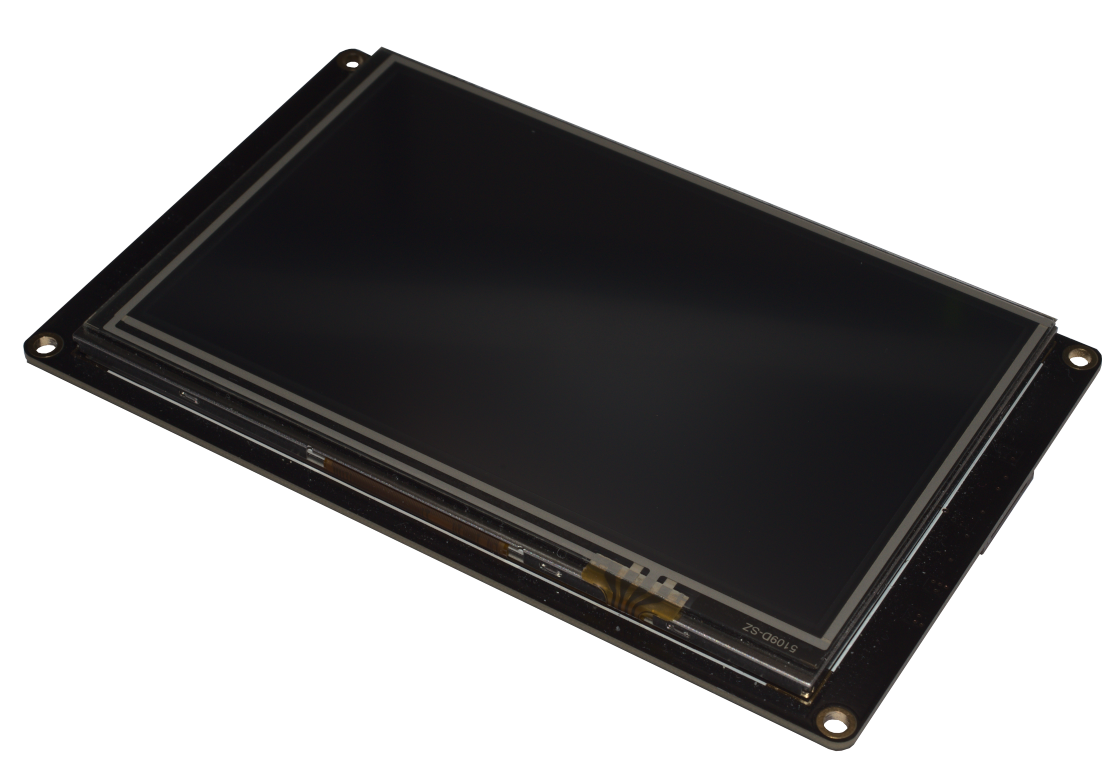
\includegraphics[width=0.8\textwidth]{Fotos/Nextion_Display.png}
    \caption{Nextion-Display}
\end{figure}
Bei dem verwendeten Bildschirm handelt es sich um einen 5 Zoll großen Touchscreen aus dem Hause Nextion.
Diese bieten den großen Vorteil, die graphische Darstellung bequem über das verfügbare gratis Tool (\textbf{Nextion Editor}) designen zu können, während der Arduino den Bildschirm nur mit den nötigen Daten über eine Serielle Verbindung versorgen muss. 

\newpage
\subsection{Installation des Nextion-Editors}
\href{https://nextion.tech/nextion-editor/}{Nextion Editor Webseite}\\
Das Programm kann entweder per heruntergeladener \textit{.exe}-Datei installiert werden, oder nach dem Entpacken der ebenfalls vorhandenen \textit{zip}-Datei direkt ausgeführt werden.
\begin{figure}[h]
    \centering
    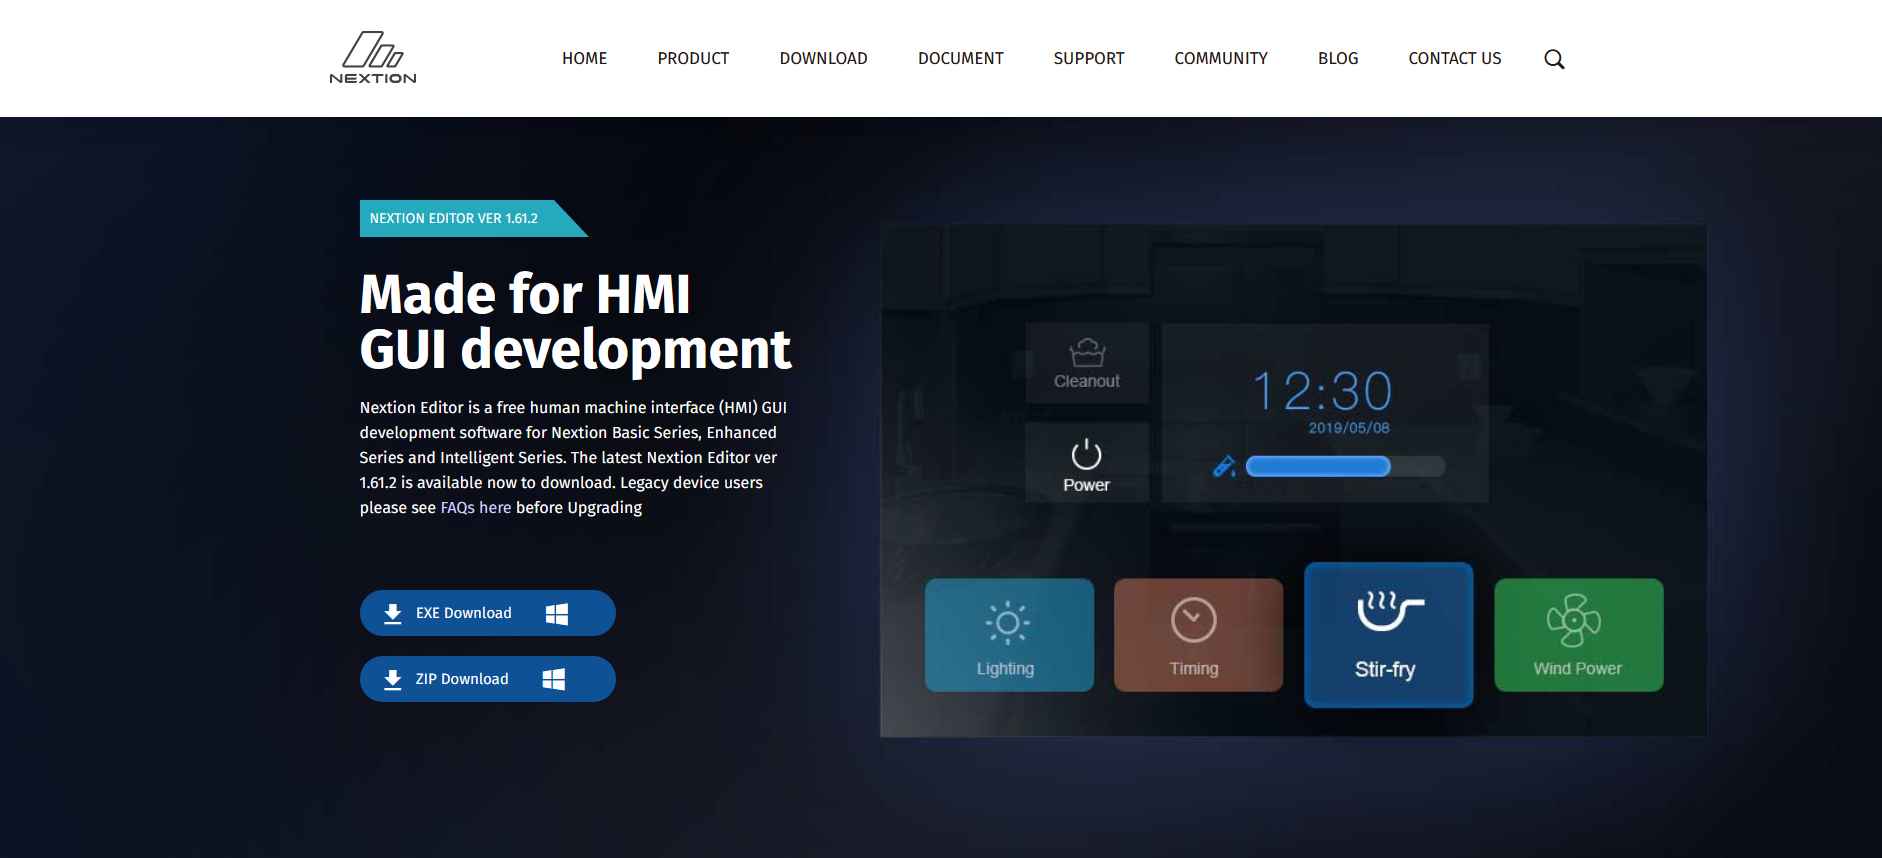
\includegraphics[width=1\textwidth]{bilder/Nextion_Webseite.png}
    \caption{Webseite des Nextion Editors}
\end{figure}

\newpage
\subsection{Auswahl des richtigen Bildschirmes}
\begin{figure}[h]
    \centering
    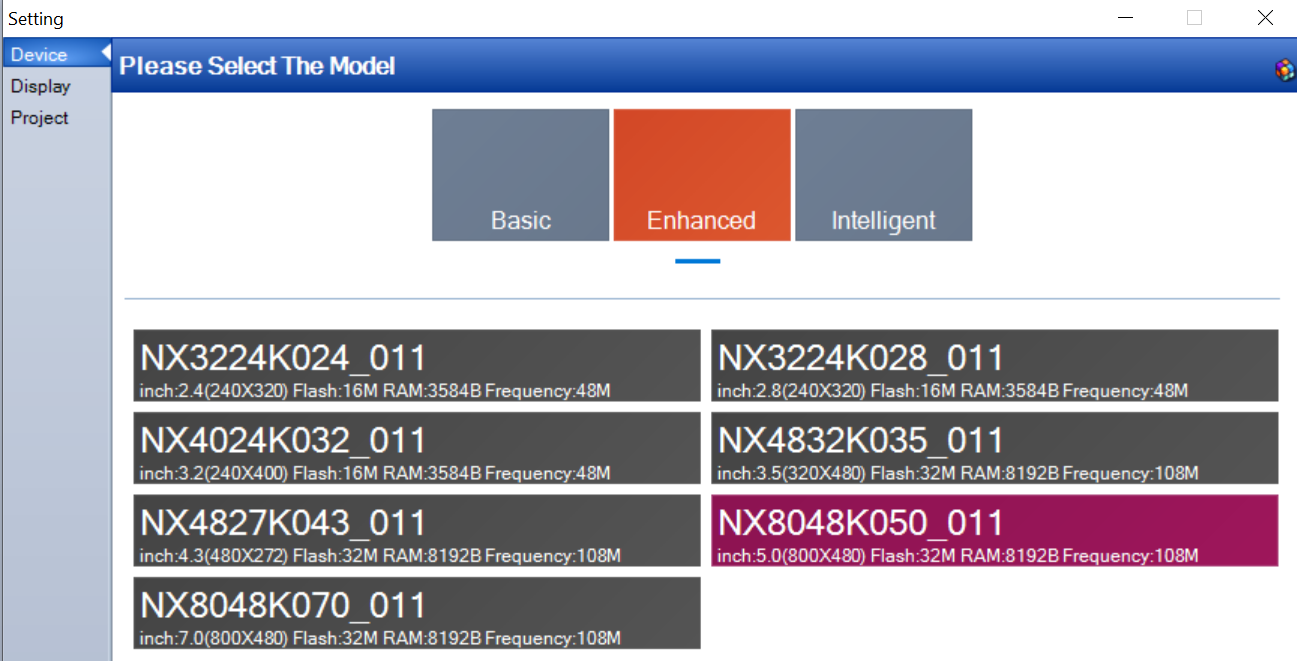
\includegraphics[width=\textwidth]{/bilder/nextion_editor/Settings_Device.png}
    \caption{Auswahl des richtigen Bildschirmes im Nextion Editor}
\end{figure}

\begin{figure}[h]
    \centering
    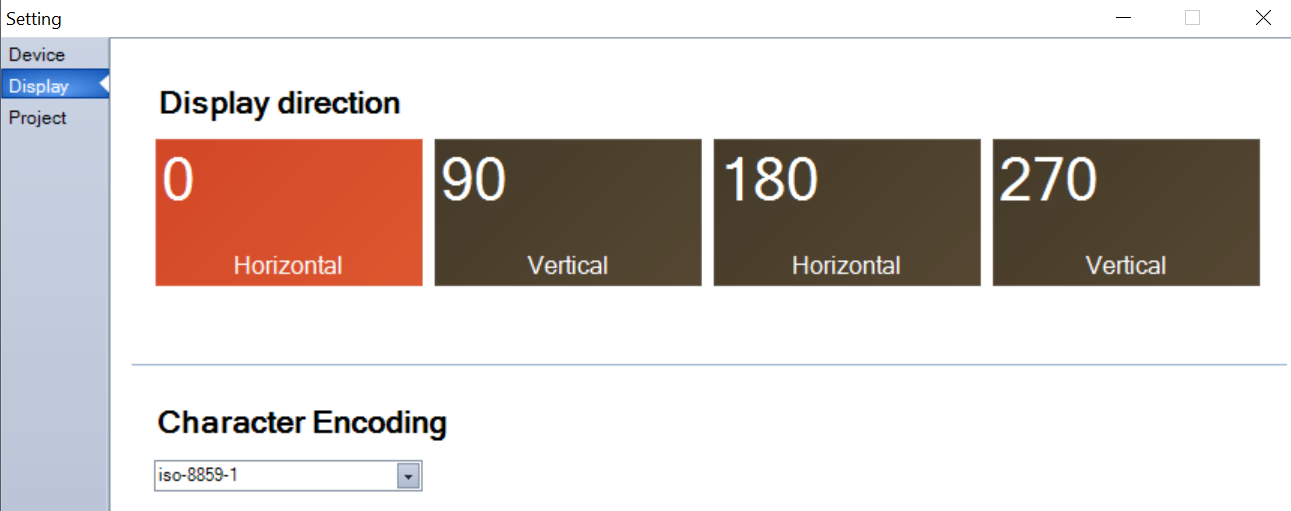
\includegraphics[width=\textwidth]{bilder/nextion_editor/Settings_Display.png}
    \caption{Auswahl des richtigen Bildschirmausrichtung im Nextion Editor}
\end{figure}

\newpage
\subsection{Entworfene Oberfläche}
\subsubsection{Hauptseite}
Diese Seite zeigt die Telemetriedaten der beiden Regler sowie die derzeitige vom GPS berechnete Geschwindigkeit an.
\begin{figure}[h]
    \centering
    %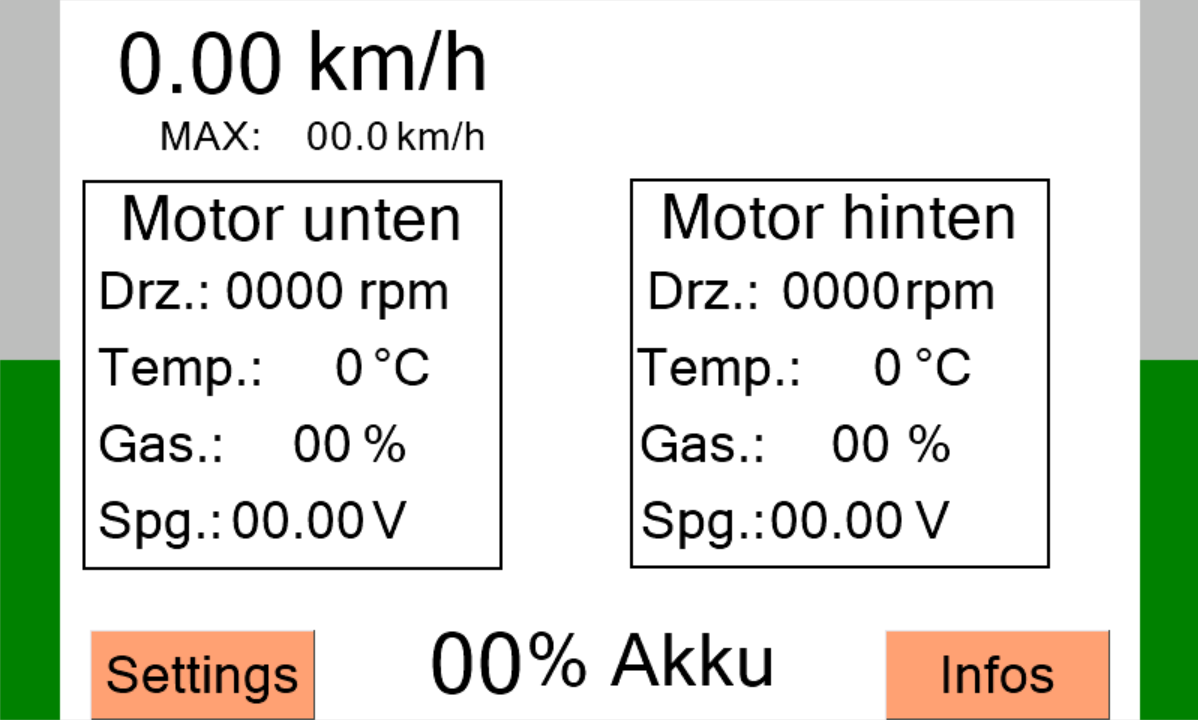
\includegraphics[width=\textwidth]{bilder/nextion_editor/main_screen.png}
    \tcbox{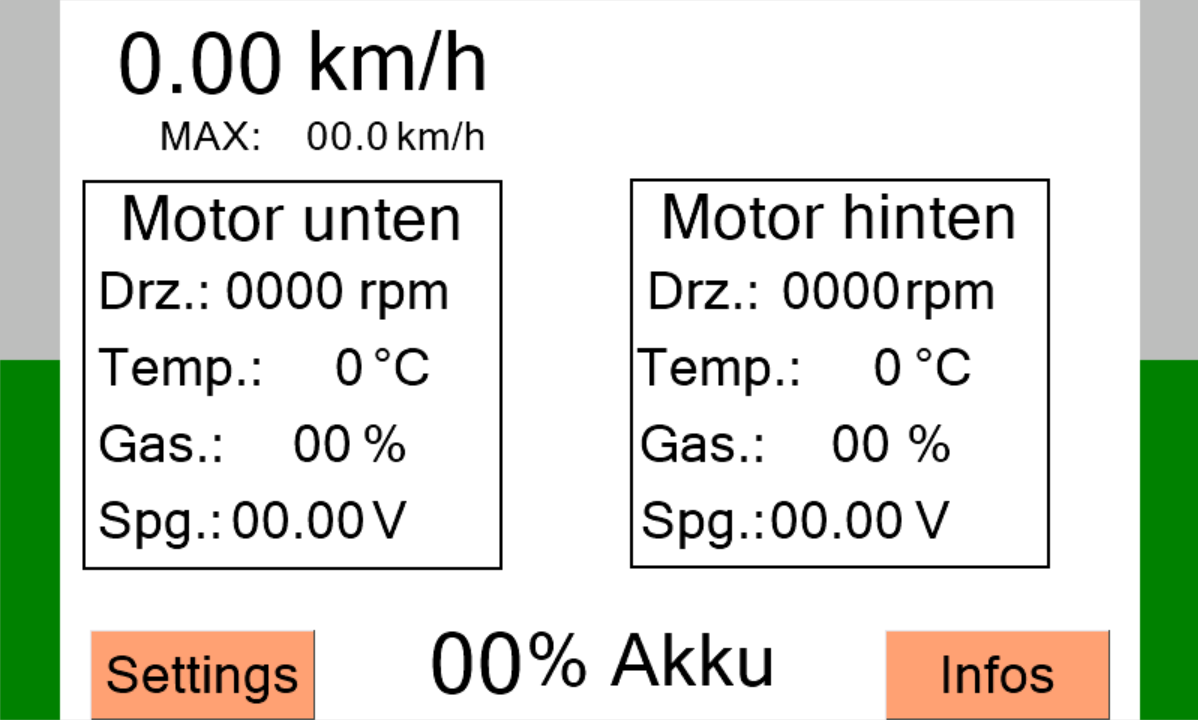
\includegraphics[width=0.9\textwidth]{bilder/nextion_editor/main_screen.png}}
    \caption{Hauptseite der Bedienoberfläche}
\end{figure}
\newpage

\subsubsection{Einstellungen}
Während man mit dem ersten Slider auf dieser Seite den Nullpunkt der Lenkung einstellen kann, 
dienen die beiden unteren Schieberegler der Begrenzung der maximal verfügbaren Leistung der beiden Motoren.
\begin{figure}[h]
    \tcbox{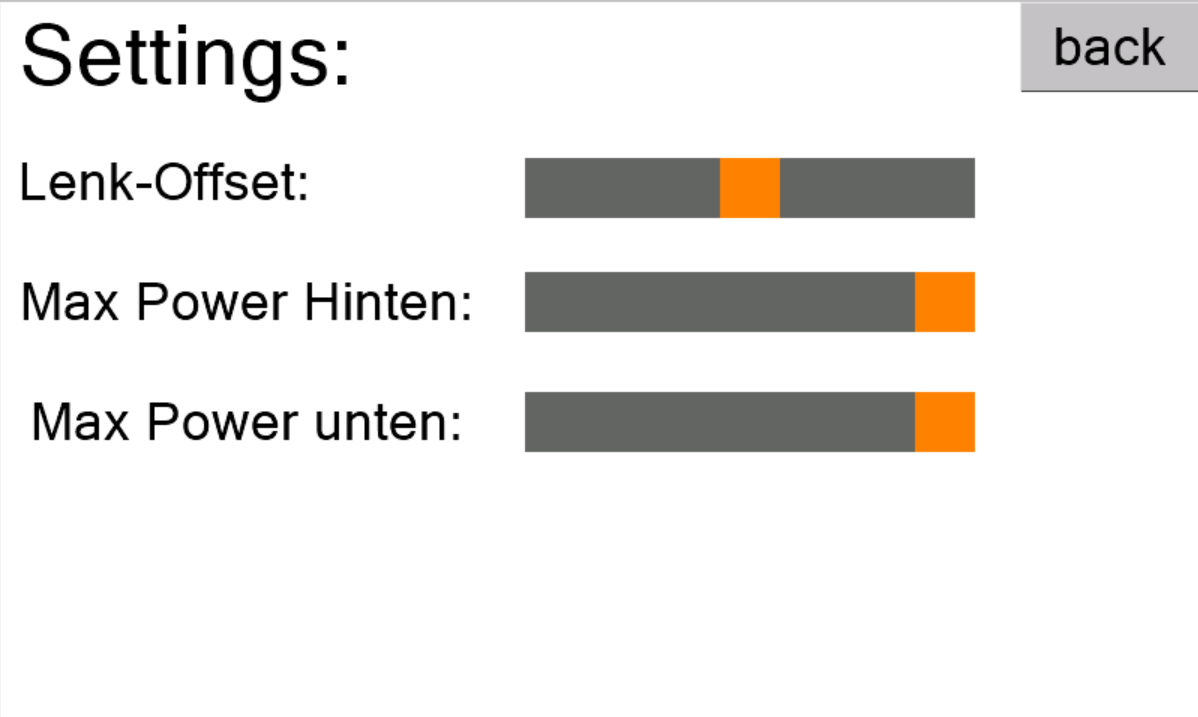
\includegraphics[width=0.9\textwidth]{bilder/nextion_editor/settings_screen.png}}
    \caption{Einstellungsseite der Bedienoberfläche}
\end{figure}
\newpage

\subsubsection{Informationen}
Diese Seite zeigt sowohl die Akkutemperaturen, als auch einige wichtigen Informationen über das GPS-Modul an.
\begin{figure}[h]
    \tcbox{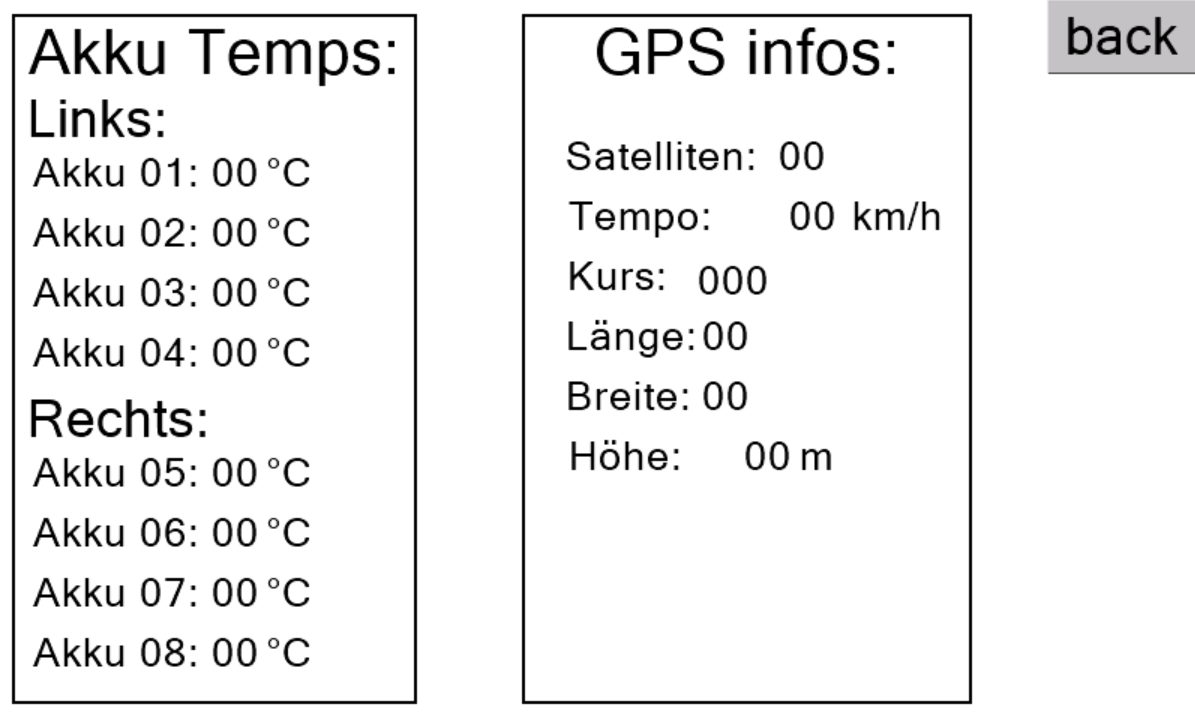
\includegraphics[width=0.9\textwidth]{bilder/nextion_editor/infos_screen.png}}
    \caption{Infoseite der Bedienoberfläche}
\end{figure}
\newpage